\chapter{Foundations}

\section{Tools}

\subsection*{Python}

Python is an interpreted, object-oriented, high-level programming language with dynamic semantics.
It is built for Rapid Application Development with and easy to learn syntax for readability.
Key features are built in data structures, dynamic typing and binding.
\cite{python-lang}
It has its own package manager called python Package Index (PyPi).
The language is compiled at execution and is available for all major platforms without charge.
The programming language is open source and maintained by the Pthon Software Foundation.
\cite{python-software-foundation}


\subsection*{NumPy}

NumPy is a package for Python.
It enables scientific computing with N-dimensional array objects and supports array broadcasting, type casting and basic linear algebra functions.
\cite{numpy-package}


\subsection*{Tensorflow}

Tensorflow is an entire ecosystem for solving problems with machine learning.
It offers multiple levels of abstraction for building, training and testing models.
For more flexibility it allows visualisations of the code and intuitive debugging.
Large machine learning training tasks can be done with distributed training on different hardware configurations without changing the model definition.
Trained models can be directly put into production.
Moreover Tensorflow offers support for multiple languages and platforms.
\cite{tensorflow-about}

\subsubsection*{Tensorflow Architecture}

\begin{figure}[H]
    \centering
    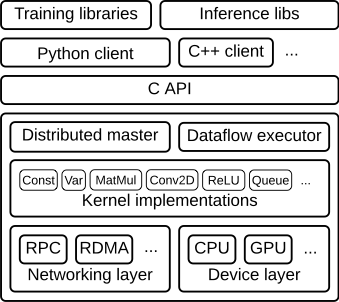
\includegraphics[scale=.5]{tensorflow_layers}
    \caption{\cite{tensorflow_layers_image} Tensorflow architecture}
    \label{fig:tensorflow_layers}
\end{figure}
The general architecture of Tensorflow is shown in figure \ref{fig:tensorflow_layers}.
It illustrates the cross-platform library.
The C API seperates the user level from the core level.
Besides the Python and C++ clients are clients for Java, JavaScript, Go, Swift, C Sharp, Haskell, Julia, Ruby, Rust and Scala available.
\cite{tensorflow-architecture}

\begin{figure}[H]
    \centering
    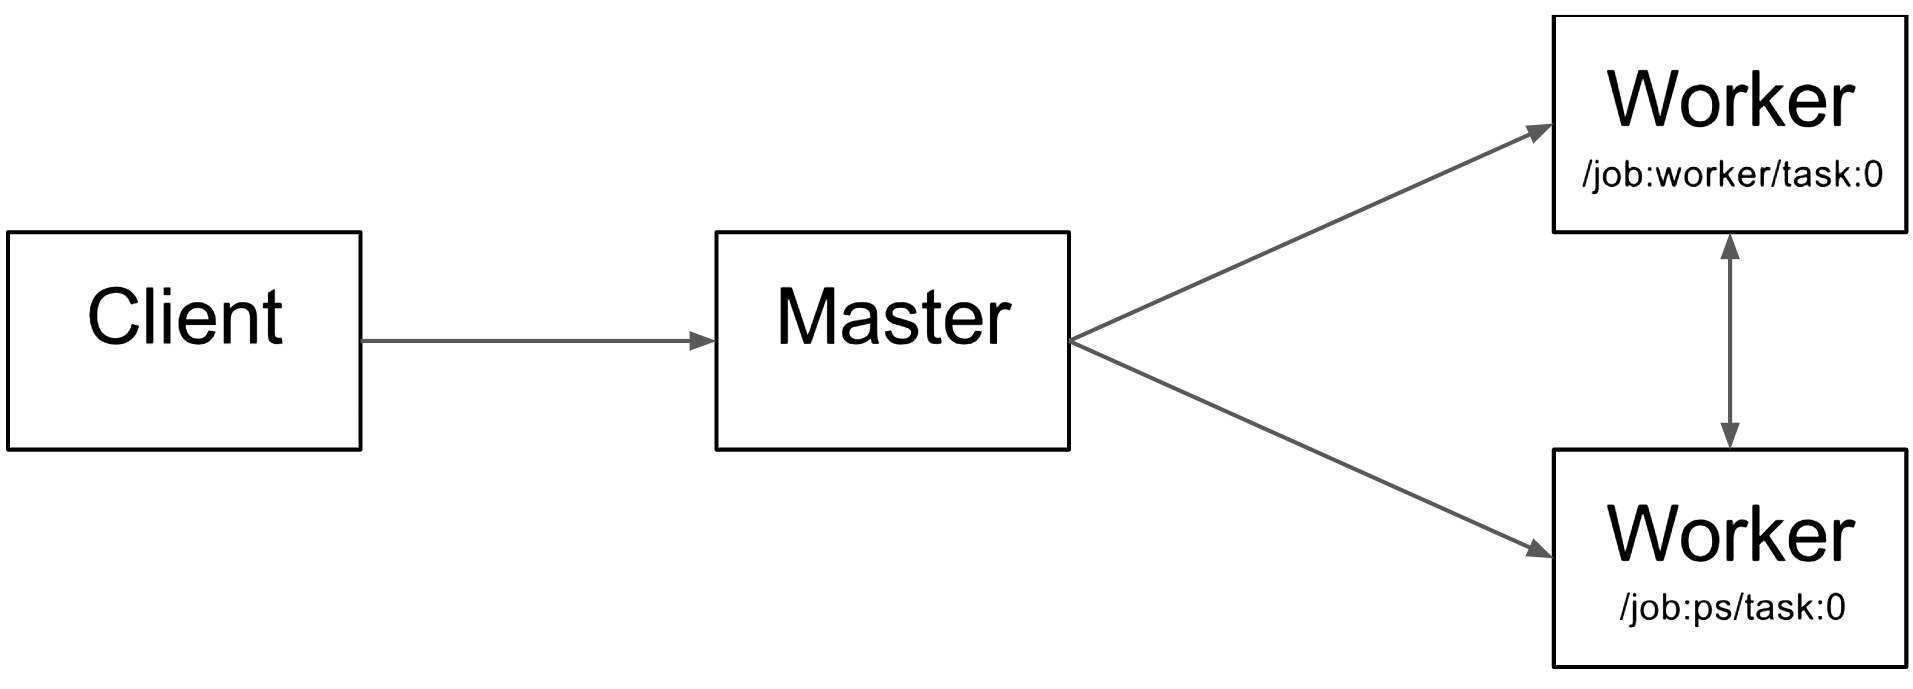
\includegraphics[width=\textwidth]{tensorflow_components}
    \caption{\cite{tensorflow_components_image} Tensorflow Components}
    \label{fig:tensorflow_components}
\end{figure}

The Client create a dataflow graph and initiates the execution by calling a session.
The Master splits the graph into multiple subgraphs and distributes these to all available workers.
The worker services use the kernel to calculate, send and receive operations from other worker services.
\cite{tensorflow-architecture}

\section{MNIST Dataset}

\begin{figure}[H]
    \centering
    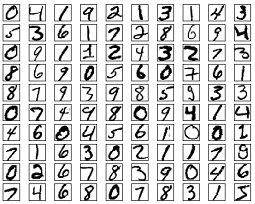
\includegraphics{mnist_100_digits}
    \caption{\cite{mnist_examples_image} Examples of handwritten digits in the mnist dataset}
    \label{fig:mnist_examples}
\end{figure}

The MNIST database is a public available dataset of handwritten digits.
It contains a set of 70,000 entities split into 60,000 training and 10,000 test parts.
The digits are size-normalized and centered photos with a fixed-size of 28 by 28 pixels.
The numbers are created by approximately 250 writers. 
\cite{mnist-database}
The Dataset pertains to one of the most popular dataset for research and testing the performance of new networks.
It is a great resource for testing new deep learning algorithms with supervised learning.

\section{Deep Neural Network}

Neural networks and deep learning currently provide the best solutions to many problems in image recognition, speech recognition, and natural language processing.
\cite{nielsen-book}
They are loosly patterned after the brain structure.
The network uses connected layers of neurons and "teaches" itself how to understand data by classifying records or making predictions.
\cite{ibm-watson-healthcare}

…

Weights are the connections between neurons.
Each weights carries a value, which shows the importance of the neuron value from the inout side.
Each weights of a neuron shape a vector.
All weights vectors from all neurons on a layer create a matrix format.

Every neuron which is not on the input layer has a bias attached.
A bias carries like every weight a value.
All bias from neurons on one layer forge a vector.

Each neuron on the hidden layers feature a activation function.

\begin{figure}[H]
    \centering
    \begin{tikzpicture}[
        init/.style={
        draw,
        circle,
        inner sep=2pt,
        font=\Huge,
        join = by -latex
        },
        squa/.style={
        draw,
        inner sep=2pt,
        font=\Large,
        join = by -latex
        },
        start chain=2,node distance=13mm
        ]
        \node[on chain=2] 
        (x2) {$x_2$};
        \node[on chain=2,join=by o-latex] 
        {$w_2$};
        \node[on chain=2,init] (sigma) 
        {$\displaystyle\Sigma$};
        \node[on chain=2,squa,label=above:{\parbox{2cm}{\centering Activation \\ function}}]
        {$f$};
        \node[on chain=2,label=above:Output,join=by -latex] 
        {$y$};
        \begin{scope}[start chain=1]
            \node[on chain=1] at (0,1.5cm) 
            (x1) {$x_1$};
            \node[on chain=1,label=above:Weights,join=by o-latex] 
            (w1) {$w_1$};
        \end{scope}
        \begin{scope}[start chain=3]
            \node[on chain=3] at (0,-1.5cm) 
            (x3) {$x_3$};
            \node[on chain=3,join=by o-latex] 
            (w3) {$w_3$};
        \end{scope}
        \node[label=above:\parbox{2cm}{\centering Bias \\ $b$}] at (sigma|-w1) (b) {};
        
        \draw[-latex] (w1) -- (sigma);
        \draw[-latex] (w3) -- (sigma);
        \draw[o-latex] (b) -- (sigma);
        
        \draw[decorate,decoration={brace,mirror}] (x1.north west) -- node[left=10pt] {Inputs} (x3.south west);
    \end{tikzpicture}
    \caption{\cite{dnn_neuron_basic_overview} Neuron structure}
    \label{fig:dnn_node_procedure}
\end{figure}

Each node on the hidden layers have a weight and bias stored. The node gets a input vector from the layer before.

\subsection*{Mathematics}

A deep neural network for classifying the mnist dataset, it uses $28*28=784$ input parameters.
The output would be for each digit (0-9) a class, which results in 10 classes.


\section{Catastrophic Forgetting}

…

\section{Elastic Weight Consolidation}

…